\documentclass[10pt]{article}

\usepackage{spheric}
%%%TITLE
\title{Modeling the melting process of quartz glass using SPH method}
\date{}

%%AFFILIATIONS
\author[$\relax$]{Zhongyi Liu}
\author[$\relax$]{Qianli Ma}
\author[$\relax$]{Haisheng Fang$^\dagger$}

\affil[$\relax$]{Huazhong University of Science \& Technology, P.R. China}

\affil[$\relax$]{\email{\dagger}{hafang@hust.edu.cn}}


%%DOCUMENT
\begin{document}

\maketitle

%\SelectedTopics{}

%%PLEASE PUT YOUR ABSTRACT HERE
\begin{abstract}
There are various complex phenomena coupled with heat transfer in melting process of quartz glass, such as large surface deformation, free surface flow and fluid-solid interaction. Smoothed Particles Hydrodynamics (SPH), a mesh-free Lagrange method, has been proved an effective tool to handle such problems. The Lagrangian framework is powerful in tracing the free interfaces by adopting the mesh-free technique to overcome the time-comsuming remeshing process in the traditional grid-based CFD method.

The goal of the present paper is to extend applications of SPH method into research of quartz glass synthesis. The process is characterized by phase transition of quartz coupled with thermal transfer and highly viscous flow. The major challenging is treatment of radiative heat transfer in SPH. In the current modeling, a strategy to simplify the radiative heat transfer is developed. During melting of quartz glass, the heater is placed at the top of the furnace. Radiative heat transfers from the heater to the high-reflective crucible inner walls, and reaches the quart ingot surfaces simultaneously. Then, the quartz ingot is heated up, and the whole surface softens. As revealed in CFD modeling, temperature at the whole surface of the quartz ingot, except the bottom, rises up almost in the same time. The radiation heating is, therefore, simplified through a heat source at the ingot surface, which depends on the view factor from the surface to the heater and the crucible inner walls, evaluated by the temperature distributions calculated in CFD models.

The Fourier law in SPH format is used to calculate thermal conduction in the system. The radiation in participating media is approximated by an effective thermal conductivity from Rosseland model. Isotherm of the softening temperature (ST) is considered as the criteria of interface of fluid and solid. In the fluid region, the physical viscosity proposed by Morris et al. (1997) is used to model low-Reynolds incompressible flows, and the Monaghan artificial viscosity is applied to solve the viscous force, respectively. Temperature-dependent viscosities are derived to denote the flow characterization of molten quartz. With the proposed models, the melting process of quartz glass is predicted, which provides an optimization tool of the quartz glass synthesis.

\begin{figure}[!htb]
\centering
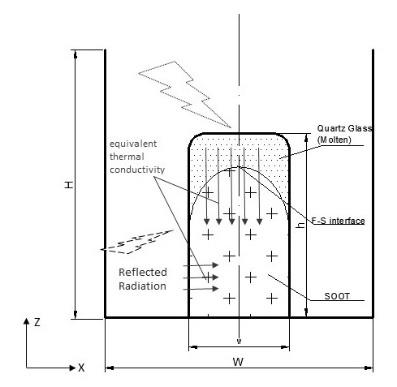
\includegraphics[width=0.4\textwidth]{25-11.png}\hspace{3em}
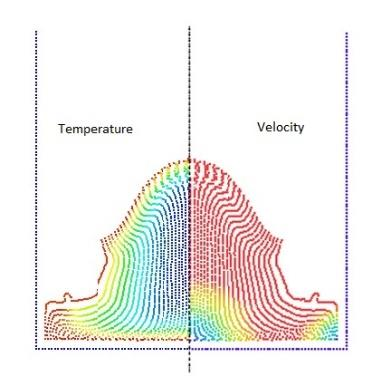
\includegraphics[width=0.4\textwidth]{25-12.png}
\caption{-Melting process simulation in SPH. Left is a sketch of melting system, and right is distribution of temperature and velocity in a moment.}\label{fig:25}
\end{figure}

\end{abstract}


%%THE END OF ABSTRACT

%\addbib

\end{document}
